% Created by tikzDevice version 0.12.6 on 2026-07-03 04:21:20
% !TEX encoding = UTF-8 Unicode
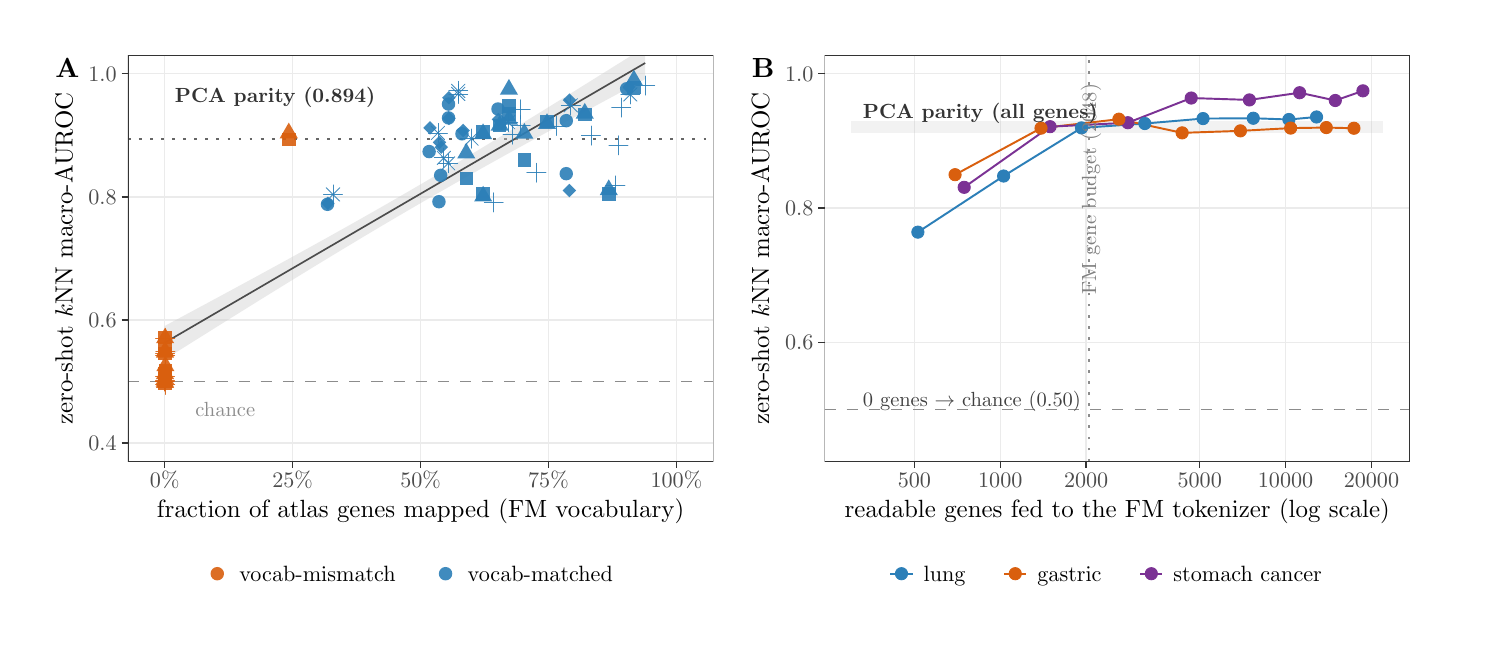
\begin{tikzpicture}[x=1pt,y=1pt]
\definecolor{fillColor}{RGB}{255,255,255}
\path[use as bounding box,fill=fillColor,fill opacity=0.00] (0,0) rectangle (517.45,216.81);
\begin{scope}
\path[clip] (  0.00,  0.00) rectangle (517.45,216.81);
\definecolor{drawColor}{RGB}{255,255,255}
\definecolor{fillColor}{RGB}{255,255,255}

\path[draw=drawColor,line width= 0.5pt,line join=round,line cap=round,fill=fillColor] (  0.00,  0.00) rectangle (517.45,216.81);
\end{scope}
\begin{scope}
\path[clip] (  5.00,  5.00) rectangle (256.73,211.81);
\definecolor{drawColor}{RGB}{255,255,255}
\definecolor{fillColor}{RGB}{255,255,255}

\path[draw=drawColor,line width= 0.5pt,line join=round,line cap=round,fill=fillColor] (  5.00,  5.00) rectangle (256.73,211.81);
\end{scope}
\begin{scope}
\path[clip] (256.73,  5.00) rectangle (508.45,211.81);
\definecolor{drawColor}{RGB}{255,255,255}
\definecolor{fillColor}{RGB}{255,255,255}

\path[draw=drawColor,line width= 0.5pt,line join=round,line cap=round,fill=fillColor] (256.73,  5.00) rectangle (508.45,211.81);
\end{scope}
\begin{scope}
\path[clip] ( 36.22, 60.07) rectangle (247.73,206.81);
\definecolor{fillColor}{RGB}{255,255,255}

\path[fill=fillColor] ( 36.22, 60.07) rectangle (247.73,206.81);
\definecolor{drawColor}{gray}{0.92}

\path[draw=drawColor,line width= 0.5pt,line join=round] ( 36.22, 66.74) --
	(247.73, 66.74);

\path[draw=drawColor,line width= 0.5pt,line join=round] ( 36.22,111.20) --
	(247.73,111.20);

\path[draw=drawColor,line width= 0.5pt,line join=round] ( 36.22,155.67) --
	(247.73,155.67);

\path[draw=drawColor,line width= 0.5pt,line join=round] ( 36.22,200.14) --
	(247.73,200.14);

\path[draw=drawColor,line width= 0.5pt,line join=round] ( 49.53, 60.07) --
	( 49.53,206.81);

\path[draw=drawColor,line width= 0.5pt,line join=round] ( 95.75, 60.07) --
	( 95.75,206.81);

\path[draw=drawColor,line width= 0.5pt,line join=round] (141.97, 60.07) --
	(141.97,206.81);

\path[draw=drawColor,line width= 0.5pt,line join=round] (188.19, 60.07) --
	(188.19,206.81);

\path[draw=drawColor,line width= 0.5pt,line join=round] (234.42, 60.07) --
	(234.42,206.81);
\definecolor{drawColor}{gray}{0.55}

\path[draw=drawColor,line width= 0.5pt,dash pattern=on 4pt off 4pt ,line join=round] ( 36.22, 88.97) -- (247.73, 88.97);
\definecolor{drawColor}{gray}{0.40}

\path[draw=drawColor,line width= 0.5pt,dash pattern=on 1pt off 3pt ,line join=round] ( 36.22,176.57) -- (247.73,176.57);
\definecolor{fillColor}{RGB}{204,204,204}

\path[fill=fillColor,fill opacity=0.40] ( 49.53,109.03) --
	( 51.73,110.21) --
	( 53.93,111.39) --
	( 56.13,112.57) --
	( 58.32,113.75) --
	( 60.52,114.93) --
	( 62.72,116.11) --
	( 64.92,117.29) --
	( 67.11,118.48) --
	( 69.31,119.66) --
	( 71.51,120.85) --
	( 73.71,122.04) --
	( 75.90,123.22) --
	( 78.10,124.42) --
	( 80.30,125.61) --
	( 82.50,126.80) --
	( 84.69,128.00) --
	( 86.89,129.20) --
	( 89.09,130.40) --
	( 91.29,131.60) --
	( 93.48,132.80) --
	( 95.68,134.01) --
	( 97.88,135.22) --
	(100.08,136.43) --
	(102.27,137.64) --
	(104.47,138.86) --
	(106.67,140.08) --
	(108.87,141.30) --
	(111.06,142.53) --
	(113.26,143.75) --
	(115.46,144.99) --
	(117.66,146.22) --
	(119.85,147.46) --
	(122.05,148.71) --
	(124.25,149.96) --
	(126.45,151.21) --
	(128.64,152.46) --
	(130.84,153.73) --
	(133.04,154.99) --
	(135.24,156.26) --
	(137.43,157.53) --
	(139.63,158.81) --
	(141.83,160.10) --
	(144.03,161.38) --
	(146.22,162.68) --
	(148.42,163.97) --
	(150.62,165.27) --
	(152.82,166.58) --
	(155.01,167.89) --
	(157.21,169.20) --
	(159.41,170.52) --
	(161.61,171.84) --
	(163.80,173.16) --
	(166.00,174.49) --
	(168.20,175.82) --
	(170.40,177.16) --
	(172.59,178.50) --
	(174.79,179.84) --
	(176.99,181.18) --
	(179.19,182.53) --
	(181.38,183.88) --
	(183.58,185.23) --
	(185.78,186.58) --
	(187.98,187.94) --
	(190.17,189.30) --
	(192.37,190.66) --
	(194.57,192.02) --
	(196.77,193.39) --
	(198.96,194.75) --
	(201.16,196.12) --
	(203.36,197.49) --
	(205.56,198.86) --
	(207.75,200.23) --
	(209.95,201.60) --
	(212.15,202.98) --
	(214.35,204.35) --
	(216.54,205.73) --
	(218.74,207.11) --
	(220.94,208.49) --
	(223.14,209.87) --
	(223.14,198.22) --
	(220.94,197.04) --
	(218.74,195.86) --
	(216.54,194.68) --
	(214.35,193.50) --
	(212.15,192.31) --
	(209.95,191.13) --
	(207.75,189.94) --
	(205.56,188.76) --
	(203.36,187.57) --
	(201.16,186.38) --
	(198.96,185.19) --
	(196.77,184.00) --
	(194.57,182.80) --
	(192.37,181.60) --
	(190.17,180.41) --
	(187.98,179.21) --
	(185.78,178.00) --
	(183.58,176.80) --
	(181.38,175.59) --
	(179.19,174.38) --
	(176.99,173.17) --
	(174.79,171.96) --
	(172.59,170.74) --
	(170.40,169.52) --
	(168.20,168.29) --
	(166.00,167.07) --
	(163.80,165.84) --
	(161.61,164.60) --
	(159.41,163.36) --
	(157.21,162.12) --
	(155.01,160.88) --
	(152.82,159.63) --
	(150.62,158.37) --
	(148.42,157.12) --
	(146.22,155.85) --
	(144.03,154.59) --
	(141.83,153.32) --
	(139.63,152.04) --
	(137.43,150.76) --
	(135.24,149.48) --
	(133.04,148.19) --
	(130.84,146.89) --
	(128.64,145.60) --
	(126.45,144.29) --
	(124.25,142.99) --
	(122.05,141.68) --
	(119.85,140.36) --
	(117.66,139.04) --
	(115.46,137.72) --
	(113.26,136.39) --
	(111.06,135.06) --
	(108.87,133.73) --
	(106.67,132.40) --
	(104.47,131.06) --
	(102.27,129.71) --
	(100.08,128.37) --
	( 97.88,127.02) --
	( 95.68,125.67) --
	( 93.48,124.32) --
	( 91.29,122.96) --
	( 89.09,121.61) --
	( 86.89,120.25) --
	( 84.69,118.89) --
	( 82.50,117.52) --
	( 80.30,116.16) --
	( 78.10,114.79) --
	( 75.90,113.42) --
	( 73.71,112.06) --
	( 71.51,110.68) --
	( 69.31,109.31) --
	( 67.11,107.94) --
	( 64.92,106.56) --
	( 62.72,105.19) --
	( 60.52,103.81) --
	( 58.32,102.43) --
	( 56.13,101.05) --
	( 53.93, 99.68) --
	( 51.73, 98.29) --
	( 49.53, 96.91) --
	cycle;

\path[] ( 49.53,109.03) --
	( 51.73,110.21) --
	( 53.93,111.39) --
	( 56.13,112.57) --
	( 58.32,113.75) --
	( 60.52,114.93) --
	( 62.72,116.11) --
	( 64.92,117.29) --
	( 67.11,118.48) --
	( 69.31,119.66) --
	( 71.51,120.85) --
	( 73.71,122.04) --
	( 75.90,123.22) --
	( 78.10,124.42) --
	( 80.30,125.61) --
	( 82.50,126.80) --
	( 84.69,128.00) --
	( 86.89,129.20) --
	( 89.09,130.40) --
	( 91.29,131.60) --
	( 93.48,132.80) --
	( 95.68,134.01) --
	( 97.88,135.22) --
	(100.08,136.43) --
	(102.27,137.64) --
	(104.47,138.86) --
	(106.67,140.08) --
	(108.87,141.30) --
	(111.06,142.53) --
	(113.26,143.75) --
	(115.46,144.99) --
	(117.66,146.22) --
	(119.85,147.46) --
	(122.05,148.71) --
	(124.25,149.96) --
	(126.45,151.21) --
	(128.64,152.46) --
	(130.84,153.73) --
	(133.04,154.99) --
	(135.24,156.26) --
	(137.43,157.53) --
	(139.63,158.81) --
	(141.83,160.10) --
	(144.03,161.38) --
	(146.22,162.68) --
	(148.42,163.97) --
	(150.62,165.27) --
	(152.82,166.58) --
	(155.01,167.89) --
	(157.21,169.20) --
	(159.41,170.52) --
	(161.61,171.84) --
	(163.80,173.16) --
	(166.00,174.49) --
	(168.20,175.82) --
	(170.40,177.16) --
	(172.59,178.50) --
	(174.79,179.84) --
	(176.99,181.18) --
	(179.19,182.53) --
	(181.38,183.88) --
	(183.58,185.23) --
	(185.78,186.58) --
	(187.98,187.94) --
	(190.17,189.30) --
	(192.37,190.66) --
	(194.57,192.02) --
	(196.77,193.39) --
	(198.96,194.75) --
	(201.16,196.12) --
	(203.36,197.49) --
	(205.56,198.86) --
	(207.75,200.23) --
	(209.95,201.60) --
	(212.15,202.98) --
	(214.35,204.35) --
	(216.54,205.73) --
	(218.74,207.11) --
	(220.94,208.49) --
	(223.14,209.87);

\path[] (223.14,198.22) --
	(220.94,197.04) --
	(218.74,195.86) --
	(216.54,194.68) --
	(214.35,193.50) --
	(212.15,192.31) --
	(209.95,191.13) --
	(207.75,189.94) --
	(205.56,188.76) --
	(203.36,187.57) --
	(201.16,186.38) --
	(198.96,185.19) --
	(196.77,184.00) --
	(194.57,182.80) --
	(192.37,181.60) --
	(190.17,180.41) --
	(187.98,179.21) --
	(185.78,178.00) --
	(183.58,176.80) --
	(181.38,175.59) --
	(179.19,174.38) --
	(176.99,173.17) --
	(174.79,171.96) --
	(172.59,170.74) --
	(170.40,169.52) --
	(168.20,168.29) --
	(166.00,167.07) --
	(163.80,165.84) --
	(161.61,164.60) --
	(159.41,163.36) --
	(157.21,162.12) --
	(155.01,160.88) --
	(152.82,159.63) --
	(150.62,158.37) --
	(148.42,157.12) --
	(146.22,155.85) --
	(144.03,154.59) --
	(141.83,153.32) --
	(139.63,152.04) --
	(137.43,150.76) --
	(135.24,149.48) --
	(133.04,148.19) --
	(130.84,146.89) --
	(128.64,145.60) --
	(126.45,144.29) --
	(124.25,142.99) --
	(122.05,141.68) --
	(119.85,140.36) --
	(117.66,139.04) --
	(115.46,137.72) --
	(113.26,136.39) --
	(111.06,135.06) --
	(108.87,133.73) --
	(106.67,132.40) --
	(104.47,131.06) --
	(102.27,129.71) --
	(100.08,128.37) --
	( 97.88,127.02) --
	( 95.68,125.67) --
	( 93.48,124.32) --
	( 91.29,122.96) --
	( 89.09,121.61) --
	( 86.89,120.25) --
	( 84.69,118.89) --
	( 82.50,117.52) --
	( 80.30,116.16) --
	( 78.10,114.79) --
	( 75.90,113.42) --
	( 73.71,112.06) --
	( 71.51,110.68) --
	( 69.31,109.31) --
	( 67.11,107.94) --
	( 64.92,106.56) --
	( 62.72,105.19) --
	( 60.52,103.81) --
	( 58.32,102.43) --
	( 56.13,101.05) --
	( 53.93, 99.68) --
	( 51.73, 98.29) --
	( 49.53, 96.91);
\definecolor{drawColor}{gray}{0.30}

\path[draw=drawColor,line width= 0.6pt,line join=round] ( 49.53,102.97) --
	( 51.73,104.25) --
	( 53.93,105.53) --
	( 56.13,106.81) --
	( 58.32,108.09) --
	( 60.52,109.37) --
	( 62.72,110.65) --
	( 64.92,111.93) --
	( 67.11,113.21) --
	( 69.31,114.49) --
	( 71.51,115.77) --
	( 73.71,117.05) --
	( 75.90,118.32) --
	( 78.10,119.60) --
	( 80.30,120.88) --
	( 82.50,122.16) --
	( 84.69,123.44) --
	( 86.89,124.72) --
	( 89.09,126.00) --
	( 91.29,127.28) --
	( 93.48,128.56) --
	( 95.68,129.84) --
	( 97.88,131.12) --
	(100.08,132.40) --
	(102.27,133.68) --
	(104.47,134.96) --
	(106.67,136.24) --
	(108.87,137.52) --
	(111.06,138.79) --
	(113.26,140.07) --
	(115.46,141.35) --
	(117.66,142.63) --
	(119.85,143.91) --
	(122.05,145.19) --
	(124.25,146.47) --
	(126.45,147.75) --
	(128.64,149.03) --
	(130.84,150.31) --
	(133.04,151.59) --
	(135.24,152.87) --
	(137.43,154.15) --
	(139.63,155.43) --
	(141.83,156.71) --
	(144.03,157.99) --
	(146.22,159.27) --
	(148.42,160.54) --
	(150.62,161.82) --
	(152.82,163.10) --
	(155.01,164.38) --
	(157.21,165.66) --
	(159.41,166.94) --
	(161.61,168.22) --
	(163.80,169.50) --
	(166.00,170.78) --
	(168.20,172.06) --
	(170.40,173.34) --
	(172.59,174.62) --
	(174.79,175.90) --
	(176.99,177.18) --
	(179.19,178.46) --
	(181.38,179.74) --
	(183.58,181.01) --
	(185.78,182.29) --
	(187.98,183.57) --
	(190.17,184.85) --
	(192.37,186.13) --
	(194.57,187.41) --
	(196.77,188.69) --
	(198.96,189.97) --
	(201.16,191.25) --
	(203.36,192.53) --
	(205.56,193.81) --
	(207.75,195.09) --
	(209.95,196.37) --
	(212.15,197.65) --
	(214.35,198.93) --
	(216.54,200.21) --
	(218.74,201.48) --
	(220.94,202.76) --
	(223.14,204.04);
\definecolor{drawColor}{RGB}{44,127,184}

\path[draw=drawColor,draw opacity=0.90,line width= 0.3pt,line join=round,line cap=round] (211.03,187.96) -- (217.91,187.96);

\path[draw=drawColor,draw opacity=0.90,line width= 0.3pt,line join=round,line cap=round] (214.47,184.51) -- (214.47,191.40);
\definecolor{fillColor}{RGB}{44,127,184}

\path[fill=fillColor,fill opacity=0.90] (201.30,189.63) --
	(204.58,183.95) --
	(198.03,183.95) --
	cycle;

\path[fill=fillColor,fill opacity=0.90] (198.87,182.94) --
	(203.74,182.94) --
	(203.74,187.81) --
	(198.87,187.81) --
	cycle;

\path[fill=fillColor,fill opacity=0.90] (193.34,190.65) --
	(195.77,193.08) --
	(198.21,190.65) --
	(195.77,188.21) --
	cycle;

\path[fill=fillColor,fill opacity=0.90] (194.63,183.20) circle (  2.43);

\path[draw=drawColor,draw opacity=0.90,line width= 0.3pt,line join=round,line cap=round] (193.84,186.32) -- (198.71,191.19);

\path[draw=drawColor,draw opacity=0.90,line width= 0.3pt,line join=round,line cap=round] (193.84,191.19) -- (198.71,186.32);

\path[draw=drawColor,draw opacity=0.90,line width= 0.3pt,line join=round,line cap=round] (192.83,188.76) -- (199.71,188.76);

\path[draw=drawColor,draw opacity=0.90,line width= 0.3pt,line join=round,line cap=round] (196.27,185.32) -- (196.27,192.20);

\path[draw=drawColor,draw opacity=0.90,line width= 0.3pt,line join=round,line cap=round] (208.94,159.79) -- (215.82,159.79);

\path[draw=drawColor,draw opacity=0.90,line width= 0.3pt,line join=round,line cap=round] (212.38,156.34) -- (212.38,163.23);

\path[fill=fillColor,fill opacity=0.90] (209.97,161.99) --
	(213.25,156.31) --
	(206.70,156.31) --
	cycle;

\path[fill=fillColor,fill opacity=0.90] (207.54,154.31) --
	(212.41,154.31) --
	(212.41,159.17) --
	(207.54,159.17) --
	cycle;

\path[fill=fillColor,fill opacity=0.90] (193.29,157.96) --
	(195.72,160.40) --
	(198.15,157.96) --
	(195.72,155.53) --
	cycle;

\path[fill=fillColor,fill opacity=0.90] (194.61,164.05) circle (  2.43);
\definecolor{drawColor}{RGB}{217,95,14}

\path[draw=drawColor,draw opacity=0.90,line width= 0.3pt,line join=round,line cap=round] ( 46.31,100.00) -- ( 53.20,100.00);

\path[draw=drawColor,draw opacity=0.90,line width= 0.3pt,line join=round,line cap=round] ( 49.76, 96.56) -- ( 49.76,103.44);
\definecolor{fillColor}{RGB}{217,95,14}

\path[fill=fillColor,fill opacity=0.90] ( 49.76, 98.36) --
	( 53.03, 92.68) --
	( 46.48, 92.68) --
	cycle;

\path[fill=fillColor,fill opacity=0.90] ( 47.32, 90.58) --
	( 52.19, 90.58) --
	( 52.19, 95.45) --
	( 47.32, 95.45) --
	cycle;
\definecolor{drawColor}{RGB}{44,127,184}

\path[draw=drawColor,draw opacity=0.90,line width= 0.3pt,line join=round,line cap=round] (164.97,153.69) -- (171.85,153.69);

\path[draw=drawColor,draw opacity=0.90,line width= 0.3pt,line join=round,line cap=round] (168.41,150.25) -- (168.41,157.13);
\definecolor{fillColor}{RGB}{44,127,184}

\path[fill=fillColor,fill opacity=0.90] (164.59,159.68) --
	(167.86,154.00) --
	(161.31,154.00) --
	cycle;

\path[fill=fillColor,fill opacity=0.90] (162.15,154.31) --
	(167.02,154.31) --
	(167.02,159.17) --
	(162.15,159.17) --
	cycle;

\path[fill=fillColor,fill opacity=0.90] (106.04,153.36) --
	(108.47,155.79) --
	(110.91,153.36) --
	(108.47,150.93) --
	cycle;

\path[fill=fillColor,fill opacity=0.90] (108.33,152.98) circle (  2.43);

\path[draw=drawColor,draw opacity=0.90,line width= 0.3pt,line join=round,line cap=round] (107.89,154.11) -- (112.76,158.97);

\path[draw=drawColor,draw opacity=0.90,line width= 0.3pt,line join=round,line cap=round] (107.89,158.97) -- (112.76,154.11);

\path[draw=drawColor,draw opacity=0.90,line width= 0.3pt,line join=round,line cap=round] (106.88,156.54) -- (113.76,156.54);

\path[draw=drawColor,draw opacity=0.90,line width= 0.3pt,line join=round,line cap=round] (110.32,153.10) -- (110.32,159.98);

\path[draw=drawColor,draw opacity=0.90,line width= 0.3pt,line join=round,line cap=round] (210.03,174.30) -- (216.91,174.30);

\path[draw=drawColor,draw opacity=0.90,line width= 0.3pt,line join=round,line cap=round] (213.47,170.86) -- (213.47,177.74);

\path[fill=fillColor,fill opacity=0.90] (164.55,182.22) --
	(167.82,176.55) --
	(161.27,176.55) --
	cycle;

\path[fill=fillColor,fill opacity=0.90] (162.12,176.65) --
	(166.98,176.65) --
	(166.98,181.52) --
	(162.12,181.52) --
	cycle;

\path[fill=fillColor,fill opacity=0.90] (146.38,175.35) --
	(148.81,177.78) --
	(151.25,175.35) --
	(148.81,172.92) --
	cycle;

\path[fill=fillColor,fill opacity=0.90] (148.61,153.92) circle (  2.43);

\path[draw=drawColor,draw opacity=0.90,line width= 0.3pt,line join=round,line cap=round] (149.51,165.38) -- (154.37,170.24);

\path[draw=drawColor,draw opacity=0.90,line width= 0.3pt,line join=round,line cap=round] (149.51,170.24) -- (154.37,165.38);

\path[draw=drawColor,draw opacity=0.90,line width= 0.3pt,line join=round,line cap=round] (148.50,167.81) -- (155.38,167.81);

\path[draw=drawColor,draw opacity=0.90,line width= 0.3pt,line join=round,line cap=round] (151.94,164.37) -- (151.94,171.25);
\definecolor{drawColor}{RGB}{217,95,14}

\path[draw=drawColor,draw opacity=0.90,line width= 0.3pt,line join=round,line cap=round] ( 46.22,104.56) -- ( 53.10,104.56);

\path[draw=drawColor,draw opacity=0.90,line width= 0.3pt,line join=round,line cap=round] ( 49.66,101.12) -- ( 49.66,108.00);
\definecolor{fillColor}{RGB}{217,95,14}

\path[fill=fillColor,fill opacity=0.90] ( 49.66,108.45) --
	( 52.94,102.78) --
	( 46.39,102.78) --
	cycle;

\path[fill=fillColor,fill opacity=0.90] ( 47.23,102.46) --
	( 52.10,102.46) --
	( 52.10,107.32) --
	( 47.23,107.32) --
	cycle;
\definecolor{drawColor}{RGB}{44,127,184}

\path[draw=drawColor,draw opacity=0.90,line width= 0.3pt,line join=round,line cap=round] (200.10,177.82) -- (206.98,177.82);

\path[draw=drawColor,draw opacity=0.90,line width= 0.3pt,line join=round,line cap=round] (203.54,174.38) -- (203.54,181.26);
\definecolor{fillColor}{RGB}{44,127,184}

\path[fill=fillColor,fill opacity=0.90] (158.48,175.22) --
	(161.76,169.54) --
	(155.21,169.54) --
	cycle;

\path[fill=fillColor,fill opacity=0.90] (156.05,159.78) --
	(160.92,159.78) --
	(160.92,164.64) --
	(156.05,164.64) --
	cycle;

\path[fill=fillColor,fill opacity=0.90] (147.03,173.61) --
	(149.46,176.05) --
	(151.89,173.61) --
	(149.46,171.18) --
	cycle;

\path[fill=fillColor,fill opacity=0.90] (149.24,163.45) circle (  2.43);

\path[draw=drawColor,draw opacity=0.90,line width= 0.3pt,line join=round,line cap=round] (147.93,167.31) -- (152.80,172.18);

\path[draw=drawColor,draw opacity=0.90,line width= 0.3pt,line join=round,line cap=round] (147.93,172.18) -- (152.80,167.31);

\path[draw=drawColor,draw opacity=0.90,line width= 0.3pt,line join=round,line cap=round] (146.93,169.75) -- (153.81,169.75);

\path[draw=drawColor,draw opacity=0.90,line width= 0.3pt,line join=round,line cap=round] (150.37,166.31) -- (150.37,173.19);
\definecolor{drawColor}{RGB}{217,95,14}

\path[draw=drawColor,draw opacity=0.90,line width= 0.3pt,line join=round,line cap=round] ( 46.19, 98.93) -- ( 53.07, 98.93);

\path[draw=drawColor,draw opacity=0.90,line width= 0.3pt,line join=round,line cap=round] ( 49.63, 95.49) -- ( 49.63,102.37);
\definecolor{fillColor}{RGB}{217,95,14}

\path[fill=fillColor,fill opacity=0.90] ( 49.63,103.23) --
	( 52.90, 97.55) --
	( 46.35, 97.55) --
	cycle;

\path[fill=fillColor,fill opacity=0.90] ( 47.19, 98.19) --
	( 52.06, 98.19) --
	( 52.06,103.05) --
	( 47.19,103.05) --
	cycle;
\definecolor{drawColor}{RGB}{44,127,184}

\path[draw=drawColor,draw opacity=0.90,line width= 0.3pt,line join=round,line cap=round] (171.76,178.17) -- (178.64,178.17);

\path[draw=drawColor,draw opacity=0.90,line width= 0.3pt,line join=round,line cap=round] (175.20,174.73) -- (175.20,181.61);
\definecolor{fillColor}{RGB}{44,127,184}

\path[fill=fillColor,fill opacity=0.90] (170.58,185.29) --
	(173.85,179.62) --
	(167.30,179.62) --
	cycle;

\path[fill=fillColor,fill opacity=0.90] (168.14,179.07) --
	(173.01,179.07) --
	(173.01,183.94) --
	(168.14,183.94) --
	cycle;

\path[fill=fillColor,fill opacity=0.90] (142.94,180.60) --
	(145.38,183.03) --
	(147.81,180.60) --
	(145.38,178.16) --
	cycle;

\path[fill=fillColor,fill opacity=0.90] (145.06,172.04) circle (  2.43);

\path[draw=drawColor,draw opacity=0.90,line width= 0.3pt,line join=round,line cap=round] (145.83,176.34) -- (150.69,181.21);

\path[draw=drawColor,draw opacity=0.90,line width= 0.3pt,line join=round,line cap=round] (145.83,181.21) -- (150.69,176.34);

\path[draw=drawColor,draw opacity=0.90,line width= 0.3pt,line join=round,line cap=round] (144.82,178.77) -- (151.70,178.77);

\path[draw=drawColor,draw opacity=0.90,line width= 0.3pt,line join=round,line cap=round] (148.26,175.33) -- (148.26,182.21);

\path[draw=drawColor,draw opacity=0.90,line width= 0.3pt,line join=round,line cap=round] (180.37,164.39) -- (187.25,164.39);

\path[draw=drawColor,draw opacity=0.90,line width= 0.3pt,line join=round,line cap=round] (183.81,160.95) -- (183.81,167.83);

\path[fill=fillColor,fill opacity=0.90] (179.47,182.38) --
	(182.74,176.70) --
	(176.19,176.70) --
	cycle;

\path[fill=fillColor,fill opacity=0.90] (177.04,166.58) --
	(181.90,166.58) --
	(181.90,171.45) --
	(177.04,171.45) --
	cycle;

\path[fill=fillColor,fill opacity=0.90] (154.94,179.66) --
	(157.37,182.10) --
	(159.81,179.66) --
	(157.37,177.23) --
	cycle;

\path[fill=fillColor,fill opacity=0.90] (156.93,178.46) circle (  2.43);

\path[draw=drawColor,draw opacity=0.90,line width= 0.3pt,line join=round,line cap=round] (157.96,174.27) -- (162.82,179.14);

\path[draw=drawColor,draw opacity=0.90,line width= 0.3pt,line join=round,line cap=round] (157.96,179.14) -- (162.82,174.27);

\path[draw=drawColor,draw opacity=0.90,line width= 0.3pt,line join=round,line cap=round] (156.95,176.71) -- (163.83,176.71);

\path[draw=drawColor,draw opacity=0.90,line width= 0.3pt,line join=round,line cap=round] (160.39,173.26) -- (160.39,180.15);

\path[draw=drawColor,draw opacity=0.90,line width= 0.3pt,line join=round,line cap=round] (174.68,187.31) -- (181.56,187.31);

\path[draw=drawColor,draw opacity=0.90,line width= 0.3pt,line join=round,line cap=round] (178.12,183.87) -- (178.12,190.75);

\path[fill=fillColor,fill opacity=0.90] (173.90,187.45) --
	(177.18,181.77) --
	(170.63,181.77) --
	cycle;

\path[fill=fillColor,fill opacity=0.90] (171.47,183.25) --
	(176.34,183.25) --
	(176.34,188.12) --
	(171.47,188.12) --
	cycle;

\path[fill=fillColor,fill opacity=0.90] (149.78,184.02) --
	(152.22,186.45) --
	(154.65,184.02) --
	(152.22,181.59) --
	cycle;

\path[fill=fillColor,fill opacity=0.90] (152.07,184.20) circle (  2.43);

\path[draw=drawColor,draw opacity=0.90,line width= 0.3pt,line join=round,line cap=round] (153.15,190.44) -- (158.01,195.30);

\path[draw=drawColor,draw opacity=0.90,line width= 0.3pt,line join=round,line cap=round] (153.15,195.30) -- (158.01,190.44);

\path[draw=drawColor,draw opacity=0.90,line width= 0.3pt,line join=round,line cap=round] (152.14,192.87) -- (159.02,192.87);

\path[draw=drawColor,draw opacity=0.90,line width= 0.3pt,line join=round,line cap=round] (155.58,189.43) -- (155.58,196.31);

\path[draw=drawColor,draw opacity=0.90,line width= 0.3pt,line join=round,line cap=round] (187.53,181.29) -- (194.41,181.29);

\path[draw=drawColor,draw opacity=0.90,line width= 0.3pt,line join=round,line cap=round] (190.97,177.84) -- (190.97,184.73);

\path[fill=fillColor,fill opacity=0.90] (187.66,185.89) --
	(190.94,180.22) --
	(184.38,180.22) --
	cycle;

\path[fill=fillColor,fill opacity=0.90] (185.23,180.45) --
	(190.09,180.45) --
	(190.09,185.32) --
	(185.23,185.32) --
	cycle;

\path[fill=fillColor,fill opacity=0.90] (167.68,183.64) --
	(170.11,186.08) --
	(172.55,183.64) --
	(170.11,181.21) --
	cycle;

\path[fill=fillColor,fill opacity=0.90] (169.95,187.42) circle (  2.43);

\path[draw=drawColor,draw opacity=0.90,line width= 0.3pt,line join=round,line cap=round] (171.16,180.23) -- (176.02,185.10);

\path[draw=drawColor,draw opacity=0.90,line width= 0.3pt,line join=round,line cap=round] (171.16,185.10) -- (176.02,180.23);

\path[draw=drawColor,draw opacity=0.90,line width= 0.3pt,line join=round,line cap=round] (170.15,182.66) -- (177.03,182.66);

\path[draw=drawColor,draw opacity=0.90,line width= 0.3pt,line join=round,line cap=round] (173.59,179.22) -- (173.59,186.10);
\definecolor{drawColor}{RGB}{217,95,14}

\path[draw=drawColor,draw opacity=0.90,line width= 0.3pt,line join=round,line cap=round] ( 46.09, 88.97) -- ( 52.97, 88.97);

\path[draw=drawColor,draw opacity=0.90,line width= 0.3pt,line join=round,line cap=round] ( 49.53, 85.53) -- ( 49.53, 92.41);
\definecolor{fillColor}{RGB}{217,95,14}

\path[fill=fillColor,fill opacity=0.90] ( 94.35,182.51) --
	( 97.63,176.84) --
	( 91.07,176.84) --
	cycle;

\path[fill=fillColor,fill opacity=0.90] ( 91.92,173.89) --
	( 96.78,173.89) --
	( 96.78,178.76) --
	( 91.92,178.76) --
	cycle;

\path[draw=drawColor,draw opacity=0.90,line width= 0.3pt,line join=round,line cap=round] ( 46.09, 88.97) -- ( 52.97, 88.97);

\path[draw=drawColor,draw opacity=0.90,line width= 0.3pt,line join=round,line cap=round] ( 49.53, 85.53) -- ( 49.53, 92.41);

\path[fill=fillColor,fill opacity=0.90] ( 49.53, 92.75) --
	( 52.81, 87.08) --
	( 46.26, 87.08) --
	cycle;

\path[fill=fillColor,fill opacity=0.90] ( 47.10, 86.54) --
	( 51.97, 86.54) --
	( 51.97, 91.40) --
	( 47.10, 91.40) --
	cycle;

\path[draw=drawColor,draw opacity=0.90,line width= 0.3pt,line join=round,line cap=round] ( 46.20, 87.73) -- ( 53.09, 87.73);

\path[draw=drawColor,draw opacity=0.90,line width= 0.3pt,line join=round,line cap=round] ( 49.64, 84.28) -- ( 49.64, 91.17);

\path[fill=fillColor,fill opacity=0.90] ( 49.64, 92.31) --
	( 52.92, 86.63) --
	( 46.37, 86.63) --
	cycle;

\path[fill=fillColor,fill opacity=0.90] ( 47.21, 85.91) --
	( 52.08, 85.91) --
	( 52.08, 90.78) --
	( 47.21, 90.78) --
	cycle;
\definecolor{drawColor}{RGB}{44,127,184}

\path[draw=drawColor,draw opacity=0.90,line width= 0.3pt,line join=round,line cap=round] (219.70,195.89) -- (226.58,195.89);

\path[draw=drawColor,draw opacity=0.90,line width= 0.3pt,line join=round,line cap=round] (223.14,192.45) -- (223.14,199.33);
\definecolor{fillColor}{RGB}{44,127,184}

\path[fill=fillColor,fill opacity=0.90] (219.05,201.61) --
	(222.33,195.94) --
	(215.77,195.94) --
	cycle;

\path[fill=fillColor,fill opacity=0.90] (216.62,192.73) --
	(221.48,192.73) --
	(221.48,197.59) --
	(216.62,197.59) --
	cycle;

\path[fill=fillColor,fill opacity=0.90] (214.88,195.40) --
	(217.31,197.84) --
	(219.75,195.40) --
	(217.31,192.97) --
	cycle;

\path[fill=fillColor,fill opacity=0.90] (216.44,194.74) circle (  2.43);

\path[draw=drawColor,draw opacity=0.90,line width= 0.3pt,line join=round,line cap=round] (215.31,190.24) -- (220.17,195.10);

\path[draw=drawColor,draw opacity=0.90,line width= 0.3pt,line join=round,line cap=round] (215.31,195.10) -- (220.17,190.24);

\path[draw=drawColor,draw opacity=0.90,line width= 0.3pt,line join=round,line cap=round] (214.30,192.67) -- (221.18,192.67);

\path[draw=drawColor,draw opacity=0.90,line width= 0.3pt,line join=round,line cap=round] (217.74,189.23) -- (217.74,196.11);
\definecolor{drawColor}{RGB}{217,95,14}

\path[draw=drawColor,draw opacity=0.90,line width= 0.3pt,line join=round,line cap=round] ( 46.19, 89.24) -- ( 53.07, 89.24);

\path[draw=drawColor,draw opacity=0.90,line width= 0.3pt,line join=round,line cap=round] ( 49.63, 85.80) -- ( 49.63, 92.68);
\definecolor{fillColor}{RGB}{217,95,14}

\path[fill=fillColor,fill opacity=0.90] ( 49.63, 95.51) --
	( 52.90, 89.84) --
	( 46.35, 89.84) --
	cycle;

\path[fill=fillColor,fill opacity=0.90] ( 47.19, 89.29) --
	( 52.06, 89.29) --
	( 52.06, 94.16) --
	( 47.19, 94.16) --
	cycle;
\definecolor{drawColor}{RGB}{44,127,184}

\path[draw=drawColor,draw opacity=0.90,line width= 0.3pt,line join=round,line cap=round] (174.68,181.60) -- (181.56,181.60);

\path[draw=drawColor,draw opacity=0.90,line width= 0.3pt,line join=round,line cap=round] (178.12,178.16) -- (178.12,185.04);
\definecolor{fillColor}{RGB}{44,127,184}

\path[fill=fillColor,fill opacity=0.90] (173.90,198.28) --
	(177.18,192.60) --
	(170.63,192.60) --
	cycle;

\path[fill=fillColor,fill opacity=0.90] (171.47,186.10) --
	(176.34,186.10) --
	(176.34,190.97) --
	(171.47,190.97) --
	cycle;

\path[fill=fillColor,fill opacity=0.90] (149.78,191.49) --
	(152.22,193.92) --
	(154.65,191.49) --
	(152.22,189.06) --
	cycle;

\path[fill=fillColor,fill opacity=0.90] (152.07,189.20) circle (  2.43);

\path[draw=drawColor,draw opacity=0.90,line width= 0.3pt,line join=round,line cap=round] (153.15,191.53) -- (158.01,196.39);

\path[draw=drawColor,draw opacity=0.90,line width= 0.3pt,line join=round,line cap=round] (153.15,196.39) -- (158.01,191.53);

\path[draw=drawColor,draw opacity=0.90,line width= 0.3pt,line join=round,line cap=round] (152.14,193.96) -- (159.02,193.96);

\path[draw=drawColor,draw opacity=0.90,line width= 0.3pt,line join=round,line cap=round] (155.58,190.52) -- (155.58,197.40);
\definecolor{drawColor}{RGB}{217,95,14}

\path[draw=drawColor,draw opacity=0.90,line width= 0.3pt,line join=round,line cap=round] ( 46.20, 98.46) -- ( 53.09, 98.46);

\path[draw=drawColor,draw opacity=0.90,line width= 0.3pt,line join=round,line cap=round] ( 49.64, 95.02) -- ( 49.64,101.90);
\definecolor{fillColor}{RGB}{217,95,14}

\path[fill=fillColor,fill opacity=0.90] ( 49.64,103.74) --
	( 52.92, 98.06) --
	( 46.37, 98.06) --
	cycle;

\path[fill=fillColor,fill opacity=0.90] ( 47.21, 96.56) --
	( 52.08, 96.56) --
	( 52.08,101.43) --
	( 47.21,101.43) --
	cycle;

\path[draw=drawColor,draw opacity=0.90,line width= 0.3pt,line join=round,line cap=round] ( 46.19, 90.86) -- ( 53.07, 90.86);

\path[draw=drawColor,draw opacity=0.90,line width= 0.3pt,line join=round,line cap=round] ( 49.63, 87.42) -- ( 49.63, 94.30);

\path[fill=fillColor,fill opacity=0.90] ( 49.63, 93.73) --
	( 52.90, 88.06) --
	( 46.35, 88.06) --
	cycle;

\path[fill=fillColor,fill opacity=0.90] ( 47.19, 87.54) --
	( 52.06, 87.54) --
	( 52.06, 92.40) --
	( 47.19, 92.40) --
	cycle;
\definecolor{drawColor}{gray}{0.55}

\node[text=drawColor,anchor=base west,inner sep=0pt, outer sep=0pt, scale=  0.74] at ( 60.63, 76.42) {chance};
\definecolor{drawColor}{gray}{0.20}

\node[text=drawColor,anchor=base west,inner sep=0pt, outer sep=0pt, scale=  0.74] at ( 53.23,189.77) {\bfseries PCA parity (0.894)};

\path[draw=drawColor,line width= 0.5pt,line join=round,line cap=round] ( 36.22, 60.07) rectangle (247.73,206.81);
\end{scope}
\begin{scope}
\path[clip] (  0.00,  0.00) rectangle (517.45,216.81);
\definecolor{drawColor}{gray}{0.30}

\node[text=drawColor,anchor=base east,inner sep=0pt, outer sep=0pt, scale=  0.80] at ( 32.17, 63.98) {0.4};

\node[text=drawColor,anchor=base east,inner sep=0pt, outer sep=0pt, scale=  0.80] at ( 32.17,108.45) {0.6};

\node[text=drawColor,anchor=base east,inner sep=0pt, outer sep=0pt, scale=  0.80] at ( 32.17,152.92) {0.8};

\node[text=drawColor,anchor=base east,inner sep=0pt, outer sep=0pt, scale=  0.80] at ( 32.17,197.38) {1.0};
\end{scope}
\begin{scope}
\path[clip] (  0.00,  0.00) rectangle (517.45,216.81);
\definecolor{drawColor}{gray}{0.20}

\path[draw=drawColor,line width= 0.5pt,line join=round] ( 33.97, 66.74) --
	( 36.22, 66.74);

\path[draw=drawColor,line width= 0.5pt,line join=round] ( 33.97,111.20) --
	( 36.22,111.20);

\path[draw=drawColor,line width= 0.5pt,line join=round] ( 33.97,155.67) --
	( 36.22,155.67);

\path[draw=drawColor,line width= 0.5pt,line join=round] ( 33.97,200.14) --
	( 36.22,200.14);
\end{scope}
\begin{scope}
\path[clip] (  0.00,  0.00) rectangle (517.45,216.81);
\definecolor{drawColor}{gray}{0.20}

\path[draw=drawColor,line width= 0.5pt,line join=round] ( 49.53, 57.82) --
	( 49.53, 60.07);

\path[draw=drawColor,line width= 0.5pt,line join=round] ( 95.75, 57.82) --
	( 95.75, 60.07);

\path[draw=drawColor,line width= 0.5pt,line join=round] (141.97, 57.82) --
	(141.97, 60.07);

\path[draw=drawColor,line width= 0.5pt,line join=round] (188.19, 57.82) --
	(188.19, 60.07);

\path[draw=drawColor,line width= 0.5pt,line join=round] (234.42, 57.82) --
	(234.42, 60.07);
\end{scope}
\begin{scope}
\path[clip] (  0.00,  0.00) rectangle (517.45,216.81);
\definecolor{drawColor}{gray}{0.30}

\node[text=drawColor,anchor=base,inner sep=0pt, outer sep=0pt, scale=  0.80] at ( 49.53, 50.51) {0\%};

\node[text=drawColor,anchor=base,inner sep=0pt, outer sep=0pt, scale=  0.80] at ( 95.75, 50.51) {25\%};

\node[text=drawColor,anchor=base,inner sep=0pt, outer sep=0pt, scale=  0.80] at (141.97, 50.51) {50\%};

\node[text=drawColor,anchor=base,inner sep=0pt, outer sep=0pt, scale=  0.80] at (188.19, 50.51) {75\%};

\node[text=drawColor,anchor=base,inner sep=0pt, outer sep=0pt, scale=  0.80] at (234.42, 50.51) {100\%};
\end{scope}
\begin{scope}
\path[clip] (  0.00,  0.00) rectangle (517.45,216.81);
\definecolor{drawColor}{RGB}{0,0,0}

\node[text=drawColor,anchor=base,inner sep=0pt, outer sep=0pt, scale=  0.90] at (141.97, 39.75) {fraction of atlas genes mapped (FM vocabulary)};
\end{scope}
\begin{scope}
\path[clip] (  0.00,  0.00) rectangle (517.45,216.81);
\definecolor{drawColor}{RGB}{0,0,0}

\node[text=drawColor,rotate= 90.00,anchor=base,inner sep=0pt, outer sep=0pt, scale=  0.90] at ( 16.20,133.44) {zero-shot $k$NN macro-AUROC};
\end{scope}
\begin{scope}
\path[clip] (  0.00,  0.00) rectangle (517.45,216.81);
\definecolor{fillColor}{RGB}{255,255,255}

\path[fill=fillColor] ( 59.01, 10.00) rectangle (224.94, 29.00);
\end{scope}
\begin{scope}
\path[clip] (  0.00,  0.00) rectangle (517.45,216.81);
\definecolor{fillColor}{RGB}{255,255,255}

\path[fill=fillColor] ( 63.51, 14.50) rectangle ( 73.51, 24.50);
\definecolor{fillColor}{RGB}{217,95,14}

\path[fill=fillColor,fill opacity=0.90] ( 68.51, 19.50) circle (  2.43);
\end{scope}
\begin{scope}
\path[clip] (  0.00,  0.00) rectangle (517.45,216.81);
\definecolor{fillColor}{RGB}{255,255,255}

\path[fill=fillColor] (146.00, 14.50) rectangle (156.00, 24.50);
\definecolor{fillColor}{RGB}{44,127,184}

\path[fill=fillColor,fill opacity=0.90] (151.00, 19.50) circle (  2.43);
\end{scope}
\begin{scope}
\path[clip] (  0.00,  0.00) rectangle (517.45,216.81);
\definecolor{drawColor}{RGB}{0,0,0}

\node[text=drawColor,anchor=base west,inner sep=0pt, outer sep=0pt, scale=  0.80] at ( 76.51, 16.74) {vocab-mismatch};
\end{scope}
\begin{scope}
\path[clip] (  0.00,  0.00) rectangle (517.45,216.81);
\definecolor{drawColor}{RGB}{0,0,0}

\node[text=drawColor,anchor=base west,inner sep=0pt, outer sep=0pt, scale=  0.80] at (159.00, 16.74) {vocab-matched};
\end{scope}
\begin{scope}
\path[clip] (  0.00,  0.00) rectangle (517.45,216.81);
\definecolor{drawColor}{RGB}{0,0,0}

\node[text=drawColor,anchor=base,inner sep=0pt, outer sep=0pt, scale=  1.00] at ( 14.35,198.85) {\bfseries A};
\end{scope}
\begin{scope}
\path[clip] (287.95, 60.07) rectangle (499.45,206.81);
\definecolor{fillColor}{RGB}{255,255,255}

\path[fill=fillColor] (287.95, 60.07) rectangle (499.45,206.81);
\definecolor{drawColor}{gray}{0.92}

\path[draw=drawColor,line width= 0.5pt,line join=round] (287.95,103.12) --
	(499.45,103.12);

\path[draw=drawColor,line width= 0.5pt,line join=round] (287.95,151.63) --
	(499.45,151.63);

\path[draw=drawColor,line width= 0.5pt,line join=round] (287.95,200.14) --
	(499.45,200.14);

\path[draw=drawColor,line width= 0.5pt,line join=round] (320.43, 60.07) --
	(320.43,206.81);

\path[draw=drawColor,line width= 0.5pt,line join=round] (351.46, 60.07) --
	(351.46,206.81);

\path[draw=drawColor,line width= 0.5pt,line join=round] (382.49, 60.07) --
	(382.49,206.81);

\path[draw=drawColor,line width= 0.5pt,line join=round] (423.51, 60.07) --
	(423.51,206.81);

\path[draw=drawColor,line width= 0.5pt,line join=round] (454.54, 60.07) --
	(454.54,206.81);

\path[draw=drawColor,line width= 0.5pt,line join=round] (485.57, 60.07) --
	(485.57,206.81);
\definecolor{fillColor}{RGB}{179,179,179}

\path[fill=fillColor,fill opacity=0.16] (297.56,178.77) rectangle (489.84,183.02);
\definecolor{drawColor}{gray}{0.55}

\path[draw=drawColor,line width= 0.5pt,dash pattern=on 4pt off 4pt ,line join=round] (287.95, 78.86) -- (499.45, 78.86);

\path[draw=drawColor,line width= 0.5pt,dash pattern=on 1pt off 3pt ,line join=round] (383.55, 60.07) -- (383.55,206.81);
\definecolor{drawColor}{RGB}{44,127,184}

\path[draw=drawColor,line width= 0.7pt,line join=round] (321.67,142.92) --
	(352.65,163.20) --
	(380.80,180.59) --
	(403.67,182.17) --
	(424.71,183.96) --
	(442.86,184.08) --
	(455.74,183.62) --
	(465.73,184.54);
\definecolor{drawColor}{RGB}{217,95,14}

\path[draw=drawColor,line width= 0.7pt,line join=round] (335.11,163.68) --
	(366.17,180.49) --
	(394.31,183.74) --
	(417.17,178.80) --
	(438.22,179.52) --
	(456.37,180.52) --
	(469.25,180.71) --
	(479.24,180.47);
\definecolor{drawColor}{RGB}{123,50,148}

\path[draw=drawColor,line width= 0.7pt,line join=round] (338.40,159.12) --
	(369.43,181.03) --
	(397.55,182.46) --
	(420.44,191.38) --
	(441.47,190.70) --
	(459.62,193.30) --
	(472.50,190.49) --
	(482.49,193.98);
\definecolor{drawColor}{RGB}{44,127,184}
\definecolor{fillColor}{RGB}{44,127,184}

\path[draw=drawColor,line width= 0.3pt,line join=round,line cap=round,fill=fillColor] (465.73,184.54) circle (  2.22);

\path[draw=drawColor,line width= 0.3pt,line join=round,line cap=round,fill=fillColor] (455.74,183.62) circle (  2.22);

\path[draw=drawColor,line width= 0.3pt,line join=round,line cap=round,fill=fillColor] (442.86,184.08) circle (  2.22);

\path[draw=drawColor,line width= 0.3pt,line join=round,line cap=round,fill=fillColor] (424.71,183.96) circle (  2.22);

\path[draw=drawColor,line width= 0.3pt,line join=round,line cap=round,fill=fillColor] (403.67,182.17) circle (  2.22);

\path[draw=drawColor,line width= 0.3pt,line join=round,line cap=round,fill=fillColor] (380.80,180.59) circle (  2.22);

\path[draw=drawColor,line width= 0.3pt,line join=round,line cap=round,fill=fillColor] (352.65,163.20) circle (  2.22);

\path[draw=drawColor,line width= 0.3pt,line join=round,line cap=round,fill=fillColor] (321.67,142.92) circle (  2.22);
\definecolor{drawColor}{RGB}{123,50,148}
\definecolor{fillColor}{RGB}{123,50,148}

\path[draw=drawColor,line width= 0.3pt,line join=round,line cap=round,fill=fillColor] (482.49,193.98) circle (  2.22);

\path[draw=drawColor,line width= 0.3pt,line join=round,line cap=round,fill=fillColor] (472.50,190.49) circle (  2.22);

\path[draw=drawColor,line width= 0.3pt,line join=round,line cap=round,fill=fillColor] (459.62,193.30) circle (  2.22);

\path[draw=drawColor,line width= 0.3pt,line join=round,line cap=round,fill=fillColor] (441.47,190.70) circle (  2.22);

\path[draw=drawColor,line width= 0.3pt,line join=round,line cap=round,fill=fillColor] (420.44,191.38) circle (  2.22);

\path[draw=drawColor,line width= 0.3pt,line join=round,line cap=round,fill=fillColor] (397.55,182.46) circle (  2.22);

\path[draw=drawColor,line width= 0.3pt,line join=round,line cap=round,fill=fillColor] (369.43,181.03) circle (  2.22);

\path[draw=drawColor,line width= 0.3pt,line join=round,line cap=round,fill=fillColor] (338.40,159.12) circle (  2.22);
\definecolor{drawColor}{RGB}{217,95,14}
\definecolor{fillColor}{RGB}{217,95,14}

\path[draw=drawColor,line width= 0.3pt,line join=round,line cap=round,fill=fillColor] (479.24,180.47) circle (  2.22);

\path[draw=drawColor,line width= 0.3pt,line join=round,line cap=round,fill=fillColor] (469.25,180.71) circle (  2.22);

\path[draw=drawColor,line width= 0.3pt,line join=round,line cap=round,fill=fillColor] (456.37,180.52) circle (  2.22);

\path[draw=drawColor,line width= 0.3pt,line join=round,line cap=round,fill=fillColor] (438.22,179.52) circle (  2.22);

\path[draw=drawColor,line width= 0.3pt,line join=round,line cap=round,fill=fillColor] (417.17,178.80) circle (  2.22);

\path[draw=drawColor,line width= 0.3pt,line join=round,line cap=round,fill=fillColor] (394.31,183.74) circle (  2.22);

\path[draw=drawColor,line width= 0.3pt,line join=round,line cap=round,fill=fillColor] (366.17,180.49) circle (  2.22);

\path[draw=drawColor,line width= 0.3pt,line join=round,line cap=round,fill=fillColor] (335.11,163.68) circle (  2.22);
\definecolor{drawColor}{gray}{0.25}

\node[text=drawColor,anchor=base west,inner sep=0pt, outer sep=0pt, scale=  0.74] at (301.83, 79.95) {0 genes $\to$ chance (0.50)};
\definecolor{drawColor}{gray}{0.50}

\node[text=drawColor,rotate= 90.00,anchor=base east,inner sep=0pt, outer sep=0pt, scale=  0.74] at (386.10,196.50) {FM gene budget (2048)};
\definecolor{drawColor}{gray}{0.20}

\node[text=drawColor,anchor=base west,inner sep=0pt, outer sep=0pt, scale=  0.74] at (301.83,183.83) {\bfseries PCA parity (all genes)};

\path[draw=drawColor,line width= 0.5pt,line join=round,line cap=round] (287.95, 60.07) rectangle (499.45,206.81);
\end{scope}
\begin{scope}
\path[clip] (  0.00,  0.00) rectangle (517.45,216.81);
\definecolor{drawColor}{gray}{0.30}

\node[text=drawColor,anchor=base east,inner sep=0pt, outer sep=0pt, scale=  0.80] at (283.90,100.36) {0.6};

\node[text=drawColor,anchor=base east,inner sep=0pt, outer sep=0pt, scale=  0.80] at (283.90,148.87) {0.8};

\node[text=drawColor,anchor=base east,inner sep=0pt, outer sep=0pt, scale=  0.80] at (283.90,197.38) {1.0};
\end{scope}
\begin{scope}
\path[clip] (  0.00,  0.00) rectangle (517.45,216.81);
\definecolor{drawColor}{gray}{0.20}

\path[draw=drawColor,line width= 0.5pt,line join=round] (285.70,103.12) --
	(287.95,103.12);

\path[draw=drawColor,line width= 0.5pt,line join=round] (285.70,151.63) --
	(287.95,151.63);

\path[draw=drawColor,line width= 0.5pt,line join=round] (285.70,200.14) --
	(287.95,200.14);
\end{scope}
\begin{scope}
\path[clip] (  0.00,  0.00) rectangle (517.45,216.81);
\definecolor{drawColor}{gray}{0.20}

\path[draw=drawColor,line width= 0.5pt,line join=round] (320.43, 57.82) --
	(320.43, 60.07);

\path[draw=drawColor,line width= 0.5pt,line join=round] (351.46, 57.82) --
	(351.46, 60.07);

\path[draw=drawColor,line width= 0.5pt,line join=round] (382.49, 57.82) --
	(382.49, 60.07);

\path[draw=drawColor,line width= 0.5pt,line join=round] (423.51, 57.82) --
	(423.51, 60.07);

\path[draw=drawColor,line width= 0.5pt,line join=round] (454.54, 57.82) --
	(454.54, 60.07);

\path[draw=drawColor,line width= 0.5pt,line join=round] (485.57, 57.82) --
	(485.57, 60.07);
\end{scope}
\begin{scope}
\path[clip] (  0.00,  0.00) rectangle (517.45,216.81);
\definecolor{drawColor}{gray}{0.30}

\node[text=drawColor,anchor=base,inner sep=0pt, outer sep=0pt, scale=  0.80] at (320.43, 50.51) {500};

\node[text=drawColor,anchor=base,inner sep=0pt, outer sep=0pt, scale=  0.80] at (351.46, 50.51) {1000};

\node[text=drawColor,anchor=base,inner sep=0pt, outer sep=0pt, scale=  0.80] at (382.49, 50.51) {2000};

\node[text=drawColor,anchor=base,inner sep=0pt, outer sep=0pt, scale=  0.80] at (423.51, 50.51) {5000};

\node[text=drawColor,anchor=base,inner sep=0pt, outer sep=0pt, scale=  0.80] at (454.54, 50.51) {10000};

\node[text=drawColor,anchor=base,inner sep=0pt, outer sep=0pt, scale=  0.80] at (485.57, 50.51) {20000};
\end{scope}
\begin{scope}
\path[clip] (  0.00,  0.00) rectangle (517.45,216.81);
\definecolor{drawColor}{RGB}{0,0,0}

\node[text=drawColor,anchor=base,inner sep=0pt, outer sep=0pt, scale=  0.90] at (393.70, 39.75) {readable genes fed to the FM tokenizer (log scale)};
\end{scope}
\begin{scope}
\path[clip] (  0.00,  0.00) rectangle (517.45,216.81);
\definecolor{drawColor}{RGB}{0,0,0}

\node[text=drawColor,rotate= 90.00,anchor=base,inner sep=0pt, outer sep=0pt, scale=  0.90] at (267.93,133.44) {zero-shot $k$NN macro-AUROC};
\end{scope}
\begin{scope}
\path[clip] (  0.00,  0.00) rectangle (517.45,216.81);
\definecolor{fillColor}{RGB}{255,255,255}

\path[fill=fillColor] (306.25, 10.00) rectangle (481.16, 29.00);
\end{scope}
\begin{scope}
\path[clip] (  0.00,  0.00) rectangle (517.45,216.81);
\definecolor{fillColor}{RGB}{255,255,255}

\path[fill=fillColor] (310.75, 14.50) rectangle (320.75, 24.50);
\definecolor{drawColor}{RGB}{44,127,184}

\path[draw=drawColor,line width= 0.7pt,line join=round] (311.75, 19.50) -- (319.75, 19.50);
\definecolor{fillColor}{RGB}{44,127,184}

\path[draw=drawColor,line width= 0.3pt,line join=round,line cap=round,fill=fillColor] (315.75, 19.50) circle (  2.22);
\end{scope}
\begin{scope}
\path[clip] (  0.00,  0.00) rectangle (517.45,216.81);
\definecolor{fillColor}{RGB}{255,255,255}

\path[fill=fillColor] (351.86, 14.50) rectangle (361.86, 24.50);
\definecolor{drawColor}{RGB}{217,95,14}

\path[draw=drawColor,line width= 0.7pt,line join=round] (352.86, 19.50) -- (360.86, 19.50);
\definecolor{fillColor}{RGB}{217,95,14}

\path[draw=drawColor,line width= 0.3pt,line join=round,line cap=round,fill=fillColor] (356.86, 19.50) circle (  2.22);
\end{scope}
\begin{scope}
\path[clip] (  0.00,  0.00) rectangle (517.45,216.81);
\definecolor{fillColor}{RGB}{255,255,255}

\path[fill=fillColor] (401.03, 14.50) rectangle (411.03, 24.50);
\definecolor{drawColor}{RGB}{123,50,148}

\path[draw=drawColor,line width= 0.7pt,line join=round] (402.03, 19.50) -- (410.03, 19.50);
\definecolor{fillColor}{RGB}{123,50,148}

\path[draw=drawColor,line width= 0.3pt,line join=round,line cap=round,fill=fillColor] (406.03, 19.50) circle (  2.22);
\end{scope}
\begin{scope}
\path[clip] (  0.00,  0.00) rectangle (517.45,216.81);
\definecolor{drawColor}{RGB}{0,0,0}

\node[text=drawColor,anchor=base west,inner sep=0pt, outer sep=0pt, scale=  0.80] at (323.75, 16.74) {lung};
\end{scope}
\begin{scope}
\path[clip] (  0.00,  0.00) rectangle (517.45,216.81);
\definecolor{drawColor}{RGB}{0,0,0}

\node[text=drawColor,anchor=base west,inner sep=0pt, outer sep=0pt, scale=  0.80] at (364.86, 16.74) {gastric};
\end{scope}
\begin{scope}
\path[clip] (  0.00,  0.00) rectangle (517.45,216.81);
\definecolor{drawColor}{RGB}{0,0,0}

\node[text=drawColor,anchor=base west,inner sep=0pt, outer sep=0pt, scale=  0.80] at (414.03, 16.74) {stomach cancer};
\end{scope}
\begin{scope}
\path[clip] (  0.00,  0.00) rectangle (517.45,216.81);
\definecolor{drawColor}{RGB}{0,0,0}

\node[text=drawColor,anchor=base,inner sep=0pt, outer sep=0pt, scale=  1.00] at (265.82,198.85) {\bfseries B};
\end{scope}
\end{tikzpicture}
